\documentclass[conference]{IEEEtran}
\IEEEoverridecommandlockouts
% The preceding line is only needed to identify funding in the first footnote. If that is unneeded, please comment it out.
\usepackage{cite}
\usepackage{amsmath,amssymb,amsfonts}
\usepackage{algorithmic}
\usepackage{graphicx}
\usepackage{textcomp}
\usepackage{xcolor}
\def\BibTeX{{\rm B\kern-.05em{\sc i\kern-.025em b}\kern-.08em
    T\kern-.1667em\lower.7ex\hbox{E}\kern-.125emX}}

\makeatletter
\def\endthebibliography{%
  \def\@noitemerr{\@latex@warning{Empty `thebibliography' environment}}%
  \endlist
}
\makeatother


\begin{document}

\title{Building GUI Application of Splitter (Mining Fine-Grained Sequential Patterns in Semantic)
Trajectories\\
%\thanks{* Corresponding Author}
}

\author{\IEEEauthorblockN{Tanjung Dion, Fawwaz Dzaky Zakiyal}
\IEEEauthorblockA{\textit{Department of Electrical and Computer Engineering} \\
\textit{Pusan National University}\\
Busan, Republic of Korea \\
\{tanjung.dn, dzakybd\}@gmail.com}}

\maketitle

\begin{abstract}
Semantic trajectory is a sequence of timestamped places wherein each place has information about spatial location and a semantic label. By mining fine-grained pattern that satisfy semantic consistency (consistent place id in each category), spatial compactness (compact area for each category) and temporal continuity (limited time constraint), it will give benefit such as urban planning and targeted advertising. This process of mining fine-grained pattern have been proposed by Zang et. al. For the final project we will re-implement the process of find fine-grained pattern in Java programing language.
\end{abstract}

\begin{IEEEkeywords}
component, formatting
\end{IEEEkeywords}

\section{Introduction}
How to mine the coarse patterns and their snippets?
How to effectively cluster the snippets given the fact that we do not know the correct number of clusters?


\section{Implementation}
\subsection{System Design}
\begin{figure}[!ht]
\centering
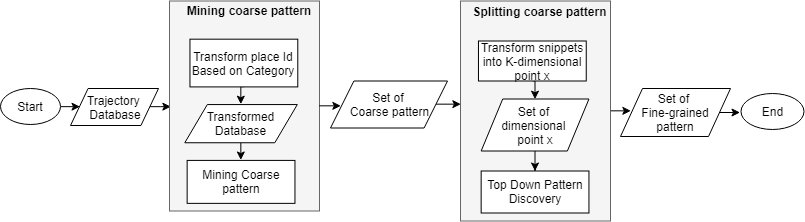
\includegraphics[width=1\linewidth]{splitter}
\caption{System Design}
\label{fig:systemdesign}
\end{figure}
Figure \ref{fig:systemdesign} show the process of mining fine-grained pattern in semantic trajectories. This method consist of two part: mining coarse pattern and splitting coarse pattern. Mining coarse pattern is a process to find sequential pattern that satisfy semantic consistency and temporal continuity. In the first step, we add trajectory dataset that have information about place id, movement time, group id, and spatial location to the system. This trajectory dataset will be transformed into semantic trajectory dataset by grouping place id based on category. However, we still keep the original place id in each category to prevent one trajectory from being counted repeatedly. By doing this process, our trajectory dataset will satisfy semantic consistency.
\par
Then, Prefixspan algorithm will be used to mining the coarse pattern. In the Prefixspan algorithm, we include all posfixes to avoid missing pattern under the given time constrain. Output from mining coarse pattern is set of coarse pattern that will be used in the next process. The next process is finding fine-grained pattern that satisfy spatial compactness in by splitting a coarse pattern in top down manner. Set of coarse pattern from previous process will be transformed into K-dimensional point x.
\par
Then, we employ mean shift clustering to extract the dense and compact snippet cluster based on the support and variance threshold. To speed up the process, the unqualified snippet cluster will be organized into several disjoint communities. By only clustering each communities, we can gradually reduce the kernel windows in clustering method to speed up the clustering process.

\subsection{Key technologies in Splitter}
Stateful Authentication has drawback that server needs to find that session and deserialize it on every request, because user data is stored on the specific server. Thus, it hard to scale, cause the server needs to create a session for a user and persist it somewhere on the server. If we have a distributed system, we have to make sure that session is shared between multiple nodes.

So, we proposed Stateless/Token Authentication where the server don't maintain the state of a user, user needs to store that token and send on every request to a restricted resource in the Authorization header. Thus, it easy to scale, cause the token contains all the information to identify the user, eliminating the need for the session state. We can pass the user to any server, instead of being bound to the same server we logged in on.
It can support high-speed mobile users, such as users in cars, users on trains, and vehicular computing. In our environment, the cloud become the auth server. Based on assumption it can guarantee the security to generate the token.

\section{Demonstration}
This document is a

\subsection{Dataset}
This project will use the real dataset, 4SQ that collected from Foursquare check-in sequence in New York. It consists of 48564 places that divided into 417 place categories and it stored semantic trajectories from 14909 users. 4SQ dataset provides 3 files:
\begin{enumerate}
\item \textit{Sequences}, it contains users semantic trajectories including attributes of check-in timestamp and place ID.
\item \textit{Places}, it contains information about the places (place ID, latitude, longitude, category ID).
\item \textit{Category}, it contains information of place category ID corresponding with its place category name.
\end{enumerate}

\subsection{Result}
We will re-implement the process of mining fine-grained pattern using java programing language. The user interface of program will be provided as shown in the Figure \ref{fig:UI}. Figure \ref{fig:javagui} shows the illustration of our program. There are an dataset input in csv format, 4 parameters input,  show button for showing graph representation like in the figure \ref{fig:graph}, and 3 button to start the process individually or start all of the process respectively. 

\begin{figure}[!ht]
\centering
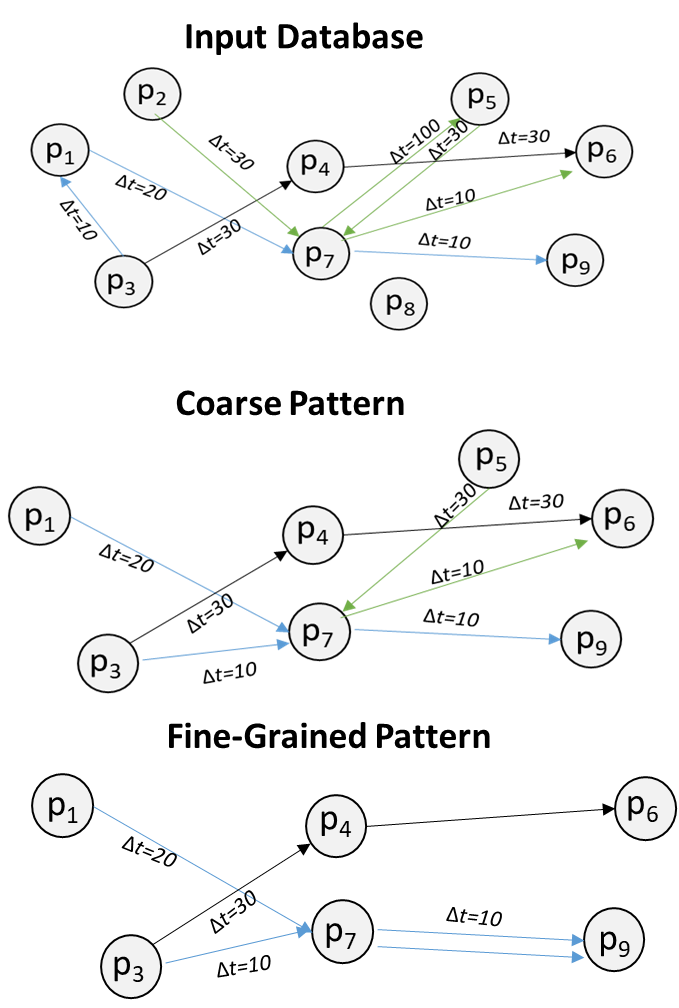
\includegraphics[width=0.5\linewidth]{GraphRepresentation}
\caption{Graph illustration}
\label{fig:graph}
\end{figure}

\begin{figure}[!ht]
\centering
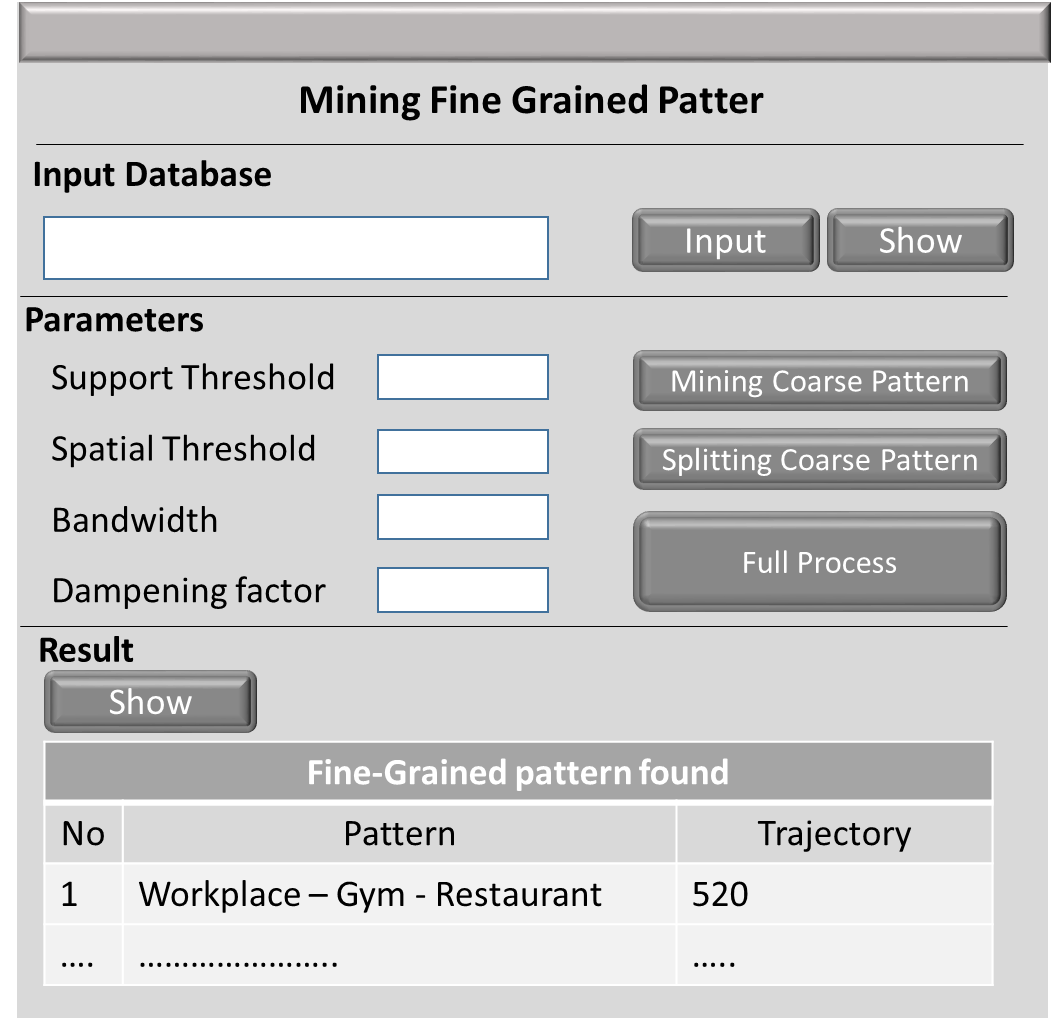
\includegraphics[width=0.5\linewidth]{GUI}
\caption{Program UI illustration}
\label{fig:javagui}
\end{figure}


This document is a \cite{sdbproject}

\section{Conclusion}
This document is a \cite{zhang2014splitter}

\section*{Acknowledgment}
This paper is submitted to fulfill term project task from Stream Database class (Fall 2018), Pusan National University.

\bibliographystyle{IEEEtran}
\bibliography{refs}

\end{document}
